\documentclass{tikzposter} % a0paper
\tikzposterlatexaffectionproofoff
\geometry{paperwidth=84.1cm,paperheight=118.8cm}
\usepackage{graphicx}
\usepackage{tikz}
\usepackage{svg}
\usetikzlibrary{automata,calc,positioning,fit,svg.path,arrows.meta,shapes.geometric,shadows}
\usetikzlibrary{matrix}
\usepackage{marvosym}
\usepackage[marvosym]{tikzsymbols}
\usepackage{amsmath}
\usepackage{amssymb}
\usepackage{booktabs}
\usepackage{bm}
\usepackage{listings}
\usepackage{pgfplots}
\usepackage{dsfont}
\usepackage{enumitem}
\usepackage{color}
\usepackage{filecontents}
\usepackage[backend=bibtex,style=numeric,sorting=none]{biblatex}

\DeclareMathOperator{\codeif}{\mathtt{:-} }

% Imperial brand colors
\definecolor{Navy}{HTML}{154C8A}
\definecolor{ImperialBlue}{RGB}{0, 62, 116}
\definecolor{LightGrey}{RGB}{235, 238, 238}
\definecolor{CoolGrey}{RGB}{157, 157, 157}
\definecolor{LightBlue}{RGB}{212, 239, 252}

% plot colors
\definecolor{pblue}{HTML}{4477AA}
\definecolor{pgreen}{HTML}{228833}
\definecolor{pred}{HTML}{EE6677}
\definecolor{pyellow}{HTML}{CCBB44}
\definecolor{pcyan}{HTML}{66CCEE}
\definecolor{pgray}{HTML}{BBBBBB}

\makeatletter
\newenvironment{customlegend}[1][]{%
	\begingroup
	% inits/clears the lists (which might be populated from previous
	% axes):
	\pgfplots@init@cleared@structures
	\pgfplotsset{#1}%
}{%
	% draws the legend:
	\pgfplots@createlegend
	\endgroup
}%

\def\addlegendimage{\pgfplots@addlegendimage}




\usetheme{Desert}

% lower bar
\usebackgroundstyle{Default}

% title
\usetitlestyle{Filled}
\colorlet{titlebgcolor}{Navy}

% block
\useblockstyle{Minimal} % Basic
\colorlet{blocktitlebgcolor}{ImperialBlue}
\colorlet{blockbodybgcolor}{LightGrey}
\colorlet{blocktitlefgcolor}{ImperialBlue}

% inner block
\useinnerblockstyle{Default}
\colorlet{innerblocktitlebgcolor}{CoolGrey}
\colorlet{innerblockbodybgcolor}{LightGrey}

\DeclareTextFontCommand{\emph}{\color{ImperialBlue}\em}

\newcommand{\midlinegraphic}[2]{%
	\raisebox{-#1/2}{\includegraphics[height=#1]{#2}}}


% ============================ Listing definitions =============================
\definecolor{codegreen}{rgb}{0,0.6,0}
\definecolor{codegray}{rgb}{0.5,0.5,0.5}
\definecolor{codepurple}{rgb}{0.58,0,0.82}
\definecolor{backcolour}{rgb}{0.95,0.95,0.92}

\lstdefinestyle{ip}{
    numberstyle=\tiny\color{codegray},
    basicstyle=\ttfamily\footnotesize,
    breakatwhitespace=false,
    breaklines=true,
    captionpos=b,
    keepspaces=true,
    numbers=left,
    numbersep=5pt,
    showspaces=false,
    showstringspaces=false,
    showtabs=false,
    tabsize=2,
    frame=single,
    numbers=none,
}
\lstset{style=ip}
% ==============================================================================

\begin{filecontents*}{sc-mdp.txt}
action(left) :- in_s_1.    action(right) :- not in_s_1.
\end{filecontents*}

\begin{filecontents*}{sc-pomdp.txt}
0.041::action(left) ; 0.959::action(right) :- left_wall_present, \+ right_wall_present.
0.581::action(left) ; 0.419::action(right) :- \+ left_wall_present, \+ right_wall_present.
\end{filecontents*}

\begin{filecontents*}{dc-asp.txt}
action(turn_right) :- a_5, a_8.
action(forward) :- a_2.
action(toggle) :- a_3.
% Definitions of each invented predicate a_i:
a_2 :- top_right_corner_wall.
a_3 :- one_step_ahead_closed_door.
a_5 :- not curr_location_open_door,
        not one_step_ahead_closed_door.
a_8 :- two_step_ahead_unseen.
\end{filecontents*}


\begin{filecontents*}{dct-asp.txt}
action(turn_right) :- a_5, a_8.
action(forward) :- not a_1, a_2.
action(toggle) :- a_3.
action(toggle) :- a_1, not a_3, a_12.
\end{filecontents*}

\begin{filecontents*}{dcot-asp.txt}
action(turn_right) :- a_5, a_8, a_11.
action(forward) :- a_2.
action(toggle) :- a_3.
action(toggle) :- not a_2, not a_3, not a_11.
\end{filecontents*}

\renewcommand{\familydefault}{\sfdefault}
\newcommand{\softmax}{\text{softmax}}
\newcommand{\mutextanh}{\text{mutex-tanh}}

%Set title authors and institute
\title{\parbox{\linewidth}{\centering\sffamily\bfseries Neural DNF-MT: A
Neuro-symbolic Approach for\\Learning Interpretable and Editable Policies}}

\institute{\sffamily
\textsuperscript{1}Imperial College London~
\textsuperscript{2}University College London
}

\author{\sffamily
Kexin Gu Baugh\textsuperscript{1}, %
Luke Dickens\textsuperscript{2}, %
and Alessandra Russo\textsuperscript{1}
}
\addbibresource{cite.bib}


\begin{document}
\maketitle

\begin{columns}

    \column{0.35}

    \block[titlecenter,bodyoffsety=1.5cm, titleoffsety=1.5cm]{\sffamily Motivation} {
        \begin{itemize}
            \item Interpretability of RL policies
                  \begin{itemize}
                      \item Important in high-stake decision making
                      \item Amenable to policy intervention
                  \end{itemize}

            \item Limitation to existing neuro-symbolic RL methods
                  \begin{itemize}
                      \item Rule templates/mode biases to restrict search space
                      \item Human-engineered predicates
                      \item Pre-trained model to extract predicates
                  \end{itemize}
        \end{itemize}
    }

    \block[titlecenter,bodyoffsety=1.5cm, titleoffsety=1.5cm]{\sffamily Neural
        DNF-MT} {

        We propose a neuro-symbolic model called
        \emph{\color{ImperialBlue}Neural DNF-MT}.

        \vspace{1em}

        {\color{ImperialBlue}\underline{\sffamily\textbf{Contributions}}}

        \begin{itemize}
            \item \textbf{Learning interpretable policy}
                  \begin{itemize}
                      \item \textbf{Differentiable learning}: trained in
                            standard deep actor-critic algorithm + predicate
                            invention without human engineering
                      \item \textbf{Interpretable}: providing logical
                            representations: probabilistic for stochastic
                            policies and bivalent for deterministic policies
                  \end{itemize}

            \item \textbf{Ability to intervene on deterministic policy
                  (represented in logic)}
                  \begin{itemize}
                      \item \textbf{Bidirectional}: inject changes made on the
                            logic representation back to the neural model,
                            without re-training
                      \item \textbf{Faster}: inference with neural DNF-MT is at
                            least 200 times faster than inference in logic
                  \end{itemize}
        \end{itemize}

        \vspace{1em}

        {\color{ImperialBlue}\underline{\sffamily\textbf{Neural DNF-based Model}}}

        \vspace{0.5em}

        The building block of a neural DNF-based model is a semi-symbolic node
        \cite{pix2rule}:

        \begin{center}
            $y = f_{\text{activation}}\left(\sum_{i=1}^{I} w_i x_i + \beta\right), $

            with $\beta = \delta \left(\max_{i=1}^{I}|w_i| - \sum_{i=1}^{I} |w_i|\right)$
        \end{center}

        $w_i \in \mathbb{R}$: trainable weights; $x_i \in [-1, 1]$: inputs

        $\beta$: bias that enforces semi-symbolic behaviour

        $\delta \in [-1, 1]$: controls the node's characteristics, which induces
        behaviour analogous to a logical conjunction (disjunction) when $\delta
            = 1 (-1)$

        $f_{\text{activation}}$: activation function that maps the output to
        $(-1, 1)$

        $y_i \in (-1, 1)$: activation of the semi-symbolic node, which
        represents its belief in a proposition

        \vspace{0.5em}

        {\color{ImperialBlue}\emph{Example}: A conjunctive node with weights
            $[6, 0, -6, 0, 0, 6]$ can be translated into a logical form of $conj
                \leftarrow a\_0, \text{not}\ a\_2, a\_5$ (zero-indexed).}

        \vspace{0.5em}

        A neural DNF model can be constructed by a conjunctive layer and a
        disjunctive layer, both with $\tanh$ activation function:

        \vspace{-1em}

        \begin{center}
            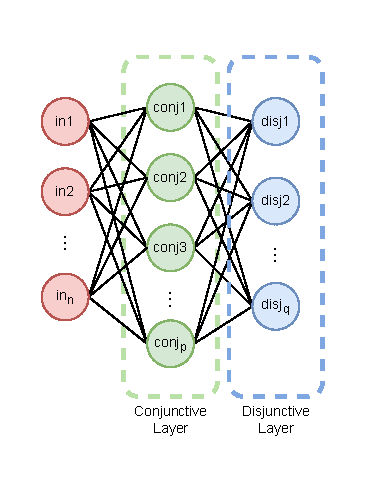
\includegraphics[width=0.6\colwidth]{img/ndnf-rl-ndnf}
        \end{center}

        \vspace{-1em}

        {\color{ImperialBlue}\underline{\sffamily\textbf{The Mutex-Tanh
                    Activation}}}

        \vspace{0.5em}

        Previous methods \cite{pix2rule,ns-classifications} used $\tanh$
        activation function in the neural DNF-based models. They do not support
        probabilistic interpretation. But for RL tasks, the model needs to
        approximate arbitrary probabilities.

        We propose a new activation function
        \emph{\color{ImperialBlue}Mutex-Tanh}:

        \begin{center}
            $\softmax(\mathbf{d})_k = e^{d_{k}} / \sum_{i}^{N} e^{d_{i}}$

            $\mutextanh(\mathbf{d})_k = 2 \cdot \softmax(\mathbf{d})_k - 1$
        \end{center}

        Mutex-tanh activation is used only at the
        disjunctive layer, while the conjunctive layer still uses $\tanh$.

    }


    % ======================================================================== %
    % ======================================================================== %
    % ======================================================================== %

    \column{0.35}

    \block[titlecenter,bodyoffsety=1.5cm, titleoffsety=1.5cm]{\sffamily Neural
        DNF-MT\\ in Actor-critic PPO} {

        \begin{center}
            \text{Usual setup for discrete observations (e.g. for two actions)}

            \vspace{-0.5em}

            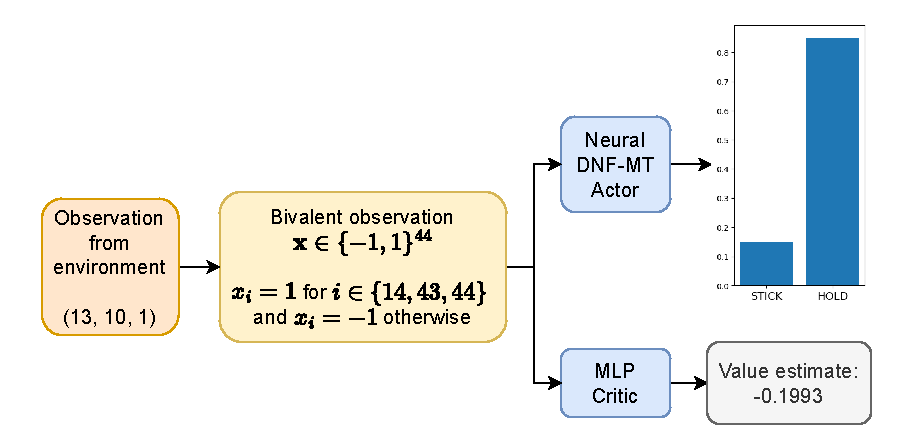
\includegraphics[width=\colwidth]{img/binary-ndnf-mt-ac}

            \text{Adaptation for predicate invention (e.g. for four actions)}

            \vspace{-0.5em}

            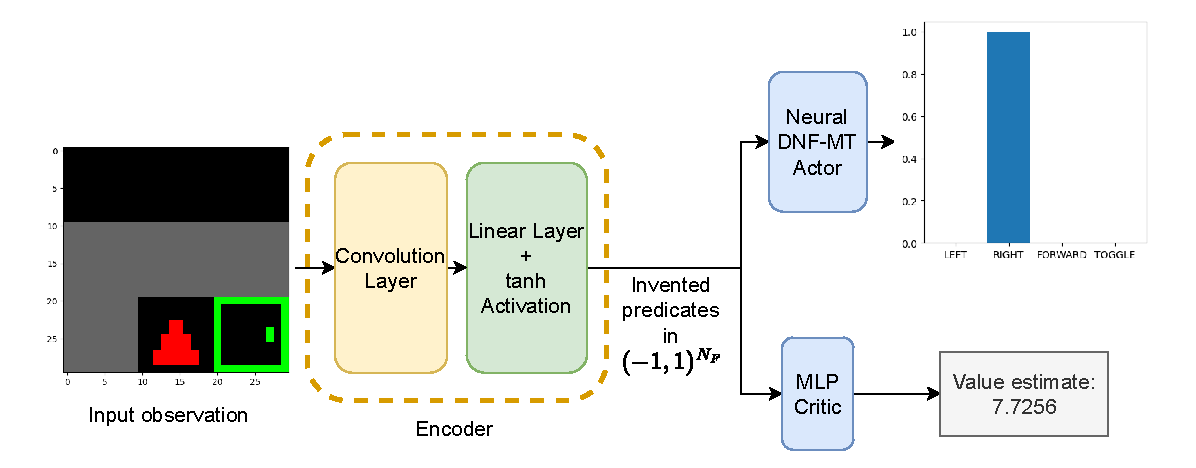
\includegraphics[width=\colwidth]{img/image-ndnf-mt-ac}

            \text{Using an \emph{\color{ImperialBlue}encoder} to extract
                meaningful symbolic features}
        \end{center}

    }

    \block[titlecenter,bodyoffsety=1.5cm, titleoffsety=1.5cm]{\sffamily
        Experiment Overview} {

        \begin{itemize}
            \item Comparable results to standard RL baselines (Q-learning \&
                  neural actor-critic PPO)
            \item In some environments, there is a trade-off between
                  interpretability and performance
        \end{itemize}

        \vspace{1em}

        *: argmax action selection, $\dagger$: $\epsilon$-greedy sampling,
        $\ddagger$: actor's distribution sampling

        \vspace{-1em}

        \begin{center}
            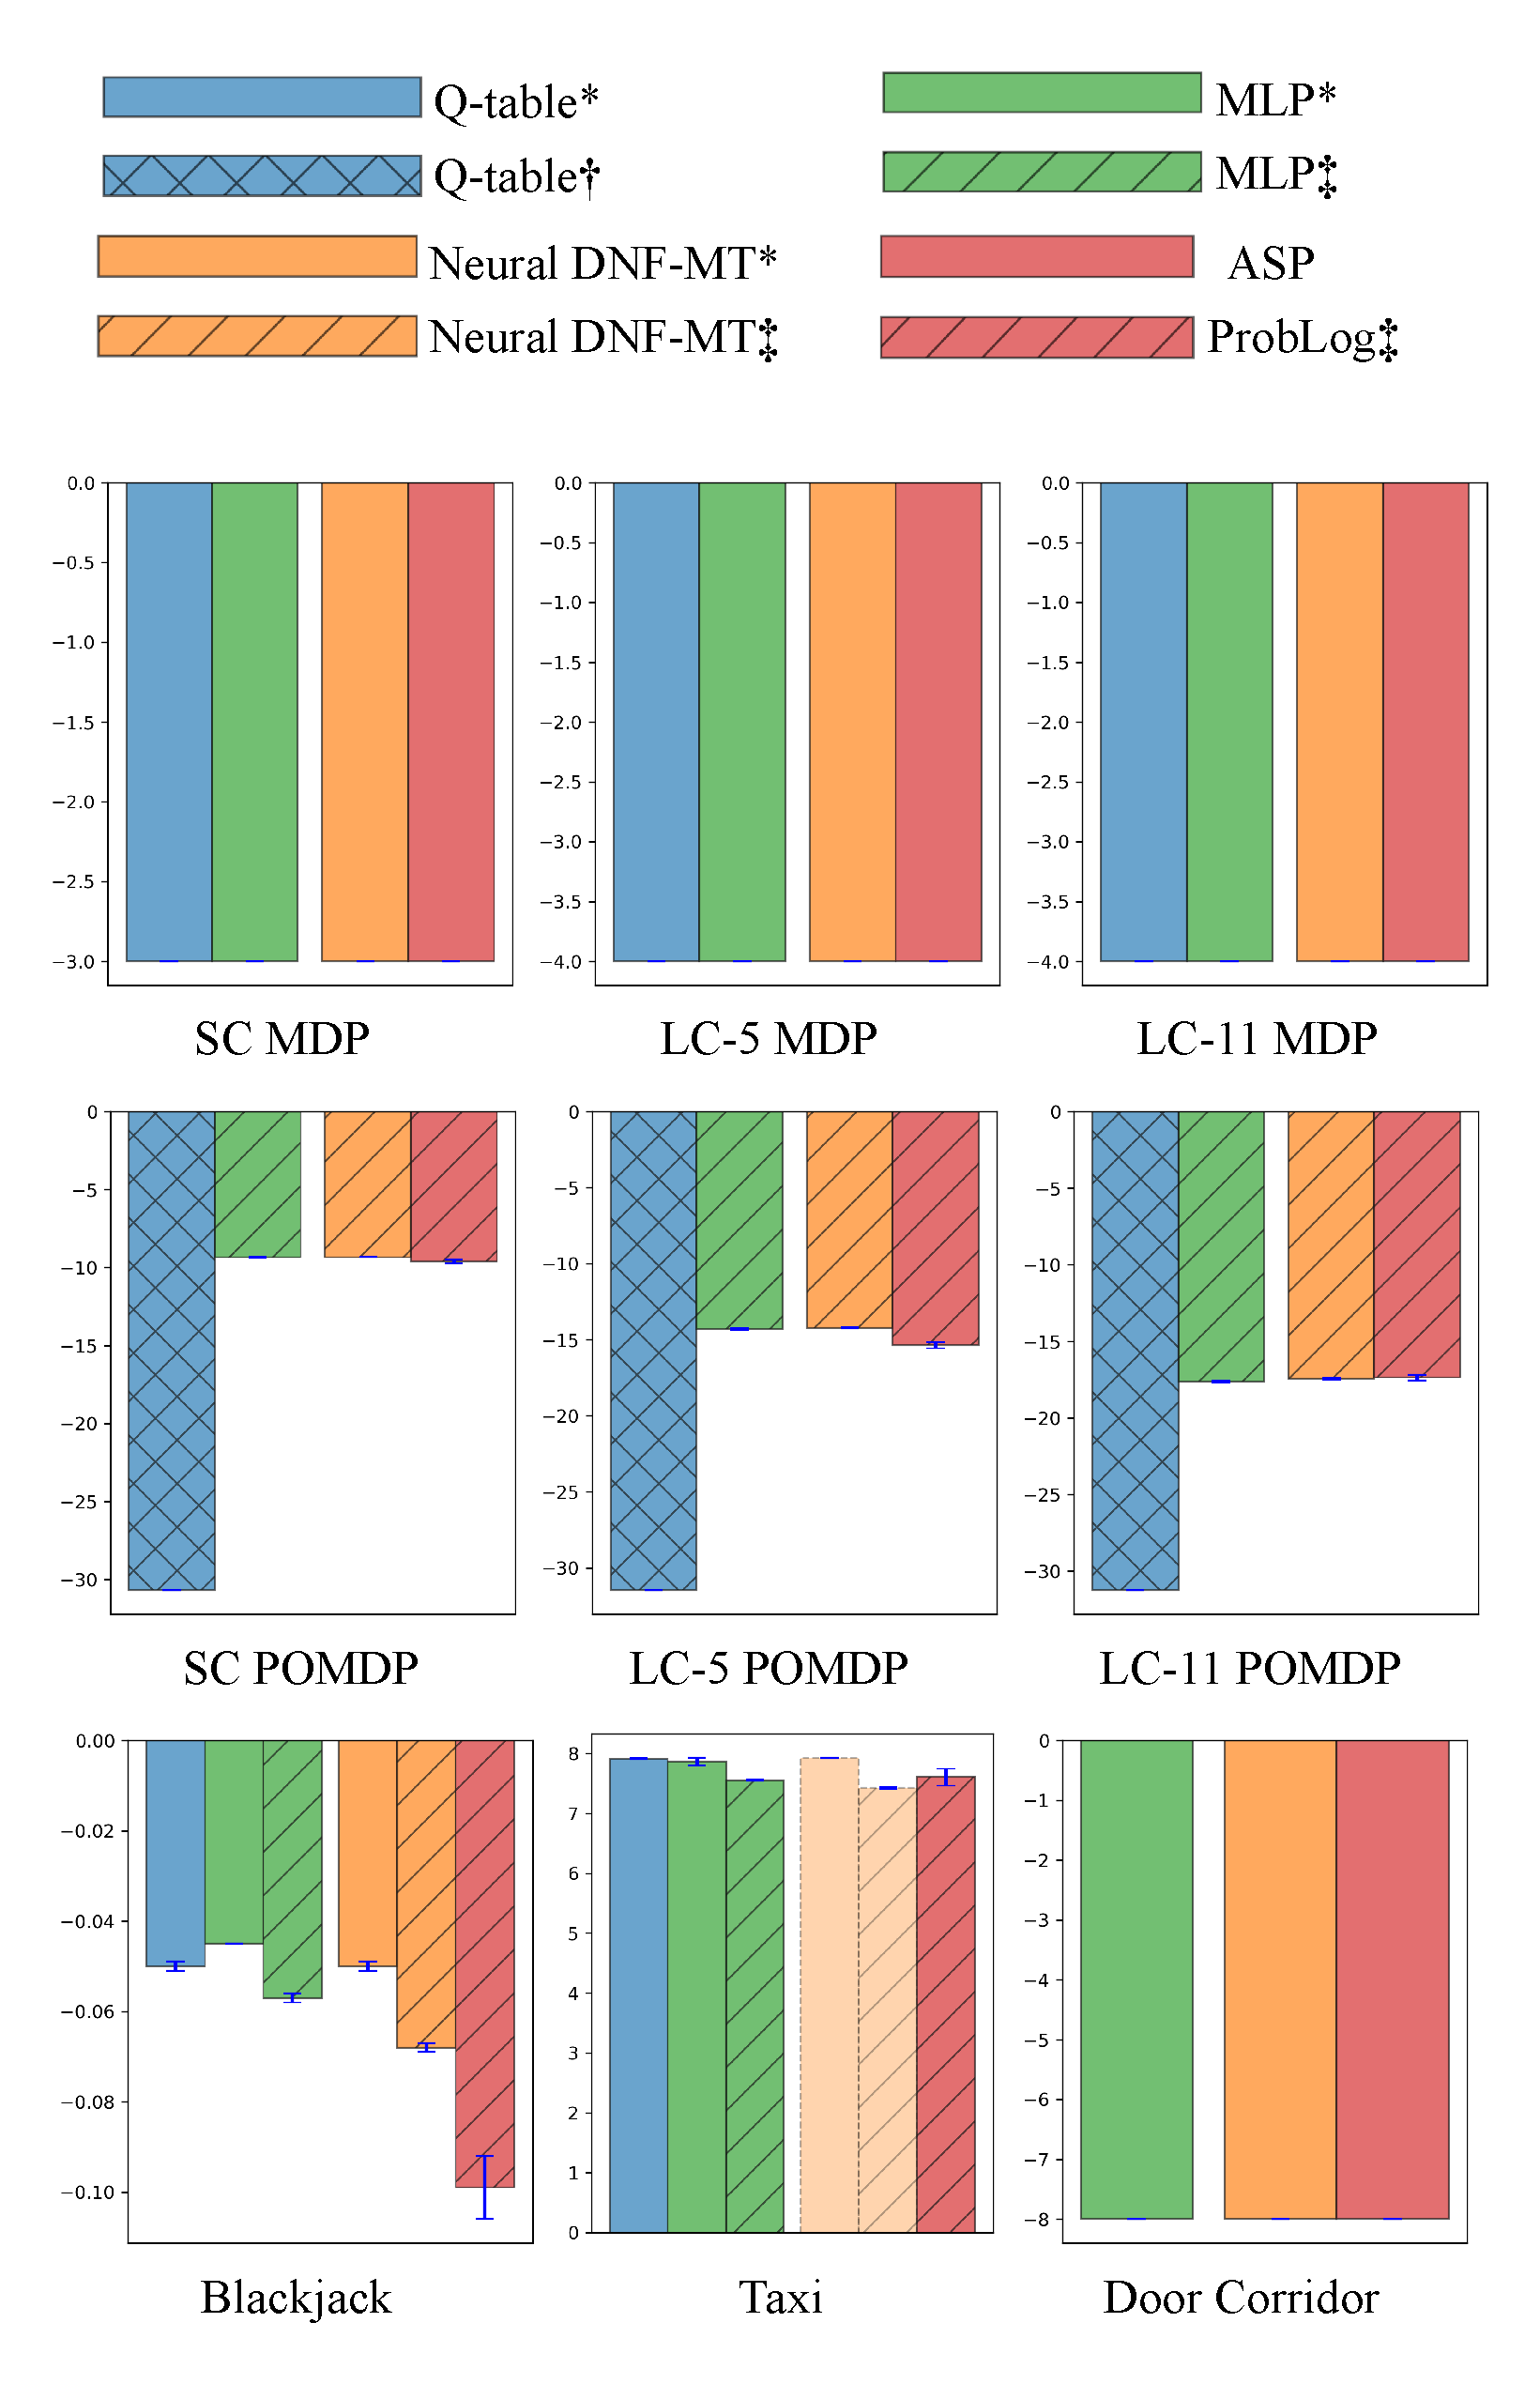
\includegraphics[width=\colwidth]{img/rl-performance}
        \end{center}

        \vspace{0.1em}

        \begin{center}
            \includegraphics[scale=0.15]{img/qr_paper.pdf}
            \hspace{30pt}
            \includegraphics[scale=0.15]{img/qr_code.pdf}

            \vspace{10pt}

            {
                \AtNextBibliography{\tiny}
                \printbibliography[heading=none]
            }
        \end{center}

    }

    % ======================================================================== %
    % ======================================================================== %
    % ======================================================================== %

    \column{0.3}

    \block[titlecenter,bodyoffsety=1.5cm, titleoffsety=1.5cm]{\sffamily Policy
        Interpretation \& Intervention} {

        {\color{ImperialBlue}\underline{\sffamily\textbf{Switcheroo Corridors}}}

        \begin{itemize}
            \item Two actions: going left and going right

            \item Reward: -1 per step

            \item Special state \emph{reverses} the agent's action

            \item Two types of observations
                  \begin{itemize}
                      \item State number (which state the agent is in):
                            \emph{MDP} \& \emph{deterministic} policy
                      \item Wall status (left and right wall): \emph{POMDP} \&
                            \emph{stochastic} policy (no memory)
                  \end{itemize}
        \end{itemize}

        \emph{Small Corridor (SC)}: 4 states, start at 0, goal at 3, special at
        1
        \begin{center}
            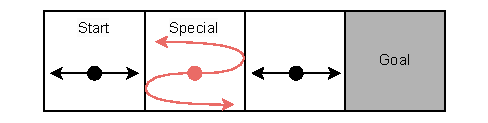
\includegraphics[width=0.8\colwidth]{img/small-corridor}
        \end{center}

        \begin{center}
            {\small ASP rules of a neural DNF-MT actor in SC MDP}
            \lstinputlisting{sc-mdp.txt}
        \end{center}

        \begin{center}
            {\small ProbLog rules of a neural DNF-MT actor in SC POMDP}
            \lstinputlisting{sc-pomdp.txt}
        \end{center}

        \vspace{0.5em}

        {\color{ImperialBlue}\underline{\sffamily\textbf{Door Corridors}}}

        \begin{itemize}
            \item Based on Key Corridor in Minigrid, but no keys, only togglable
                  doors

            \item Four actions: turn left, turn right, move forward, and toggle

            \item Agent observes a 3x3 grid around itself
        \end{itemize}

        \begin{center}
            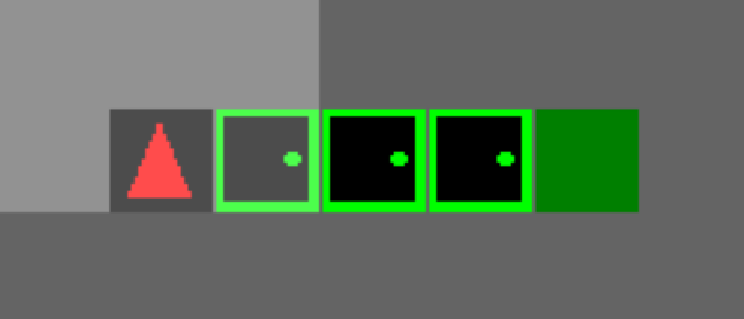
\includegraphics[width=0.8\colwidth]{img/door-corridor}
        \end{center}

        \begin{center}
            {\small ASP rules of a neural DNF-MT actor in Door Corridor}
            \lstinputlisting{dc-asp.txt}
        \end{center}
        Actions for Door Corridor: right, toggle, forward, toggle, forward,
        toggle, forward, forward

        \vspace{1em}

        \underline{\emph{Policy Modification in Modified Door Corridor}}

        \vspace{0.3em}

        We change how the agent interacts with the goal state: instead of
        stepping into the goal (Door Corridor), it needs to toggle it (DC-T).

        Instead of re-training, we adapt the existing policy:

        \begin{center}
            {\small ASP rules of a neural DNF-MT actor in DC-T}
            \lstinputlisting{dct-asp.txt}
        \end{center}

        Actions for DC-T: right, toggle, forward, toggle, forward, toggle,
        forward, \emph{toggle}

    }

    \block[titlecenter,bodyoffsety=1.5cm, titleoffsety=1.5cm]{\sffamily
        Discussion } {

        \begin{itemize}
            \item \textbf{Performance}: Comparable to standard RL baselines
                  (Q-learning \& neural actor-critic PPO)

            \item \textbf{Interpretability}: Two forms of interpretability
                  in probabilistic and bivalent logic

            \item \textbf{Inference}: Support both neural + symbolic
                  inference, and neural is faster

            \item \textbf{Policy intervention}: Edit bivalent logic program,
                  port back to neural model

            \item \textbf{Future work}: Can be helpful if there’s background
                  knowledge: provide a hot-start for training

        \end{itemize}

        \begin{center}
            
\includegraphics[scale=1]{img/aamas2025logo.png}
            
\includegraphics[scale=0.4]{img/spike_logo.png}
            
\includegraphics[width=0.1\columnwidth]{img/imperial_blue.png}
        \end{center}
    }



\end{columns}
\end{document}
